% case overview

Finding appropriate candidates for open innovation case studies proved challenging. Because this study is part of a broader initiative looking at innovation in the food and agriculture sector, cases had to be recruited from this sector. A number of potential candidates were identified using leads provided by agricultural consultants, university researchers, government agencies, and non-governmental organisations. Most of the firms approached were not keen on outsiders observing how they went about collaborative innovation. Some of these firms argued their inter-organisational relationships were a trade-secret and did not want to risk anyone finding out about their strategic intentions. Other firms felt this study would consume too much their time or be too disruptive to their operations. Ultimately, the recruitment of cases relied on a combination of perseverance and goodwill. Despite not having the luxury of choice, the three cases that were eventually recruited for this study are interesting and quite different from each other. A brief description of each case is given below. The descriptions are based on information gleaned from semi-structured interviews. Names and locations have been altered to protect the identity of firms and hide the geographic markets they operate in. \medskip

\section{Case One}

Case One examines knowledge sharing behaviour between eighteen people from seven organisations involved in a collaboration addressing cold-chain innovation. FarmCo is a family-owned business that supplies a range of green leafy vegetable products to caterers, restaurants, green grocers and supermarket chains. Products are supplied in cartons or in pre-packaged bags sold by the carton. The pre-packaged bags are supplied either as their own branded product or as a supermarket private-label product. FarmCo is based in a region that enjoys a temperate climate, enabling them to grow a greater variety of green leafy vegetables all year round. FarmCo competes with a handful of other firms for supply contracts with national supermarket chains. It views itself as a progressive business that combines innovation, expertise, and a good work ethic to provide the highest quality fresh produce to its customers.\medskip

Because green leafy vegetable products have a shelf-life of eight days post-production, FarmCo have to deliver products by refrigerated trucks to customers within two to three days of harvesting. Cartons are packed on wooden pallets stacked in two rows down the length of the refrigerated compartment. Maintaining uniform air temperatures between 1\si{\degree}C and 4\si{\degree}C in tightly-packed trucks is challenging. Refrigerated air tends to flows around the outside of a load and not through the load resulting in an uneven temperature distribution, which can lead to spoilage. FarmCo have initiated a program to improve on-farm product handling and packaging practices in an effort to reduce spoilage and improve the shelf-life of their products. The cold chain initiative is being driven by the general manager responsible for product processing and delivery at FarmCo. His goal is to ensure FarmCo is at the forefront of current best practice. FarmCo has excellent working relations with its freight forwarders, all of whom are keen to help the company improve on-farm product handling and packaging practices. The freight forwarders have a wealth of experience in cold chain logistics and are motivated to help FarmCo in order to maintain goodwill and avoid being penalised when products get rejected because of temperature issues. It is not always clear if rejections are a result of poor on-farm practices or because air temperatures were not properly maintained during transit. Working together and sharing practical knowledge is in everybody's best interest.\medskip

FarmCo uses advanced wireless micro-sensor technology provided by SensorCo to gain insight into air temperature variation inside loaded trucks. SensorCo is a foreign-based firm that specialises in monitoring the condition of perishable goods through the supply chain. They develop, manufacture, and sell miniaturised wireless sensor devices that can be placed inside individual food packages. Each device records time and temperature on a continuous basis for up to 30 days. Data can be retrieved from each device using wireless data readers up to 100m away and uploaded to a central database, where it can be queried in a variety of ways. SensorCo is helping FarmCo develop an independent monitoring system to identify problem shipments before they are unloaded. FarmCo have also enlisted the local university to model temperature distributions inside refrigerated trucks using the data provided by the wireless sensor devices. The university recently established a research group to investigate how sensor technology and data analytics can be combined to solve practical problems in perishable goods supply chains. FarmCo hope the modelling done by the research group will lead to better load configurations and packaging material to improve product performance.\medskip

The cold chain initiative involves both process and product performance innovation (Figure \ref{fig:innovationtypes}). Because the aim is to improve on-farm product handling and packaging practices, this case may be considered an example of incremental innovation. Though the cold chain initiative is ongoing, this case study focuses on knowledge sharing and creative interaction around the temperature modelling activity. FarmCo see this initiative as their first serious foray into open innovation and are keen to improve their knowledge sharing practices.\medskip

\section{Case Two}

This case examines knowledge sharing behaviour between 25 people from 8 organisations involved in a collaboration around farm system innovation. Dairy farming is a very demanding business. Not only do farmers have to work long hours, they also have to deal with market volatility that makes running a profitable dairy operation very difficult. Many dairy farmers are looking at innovative ways to sustain their operations.\medskip

MilkTech is a multinational firm specialising in state-of-the-art dairy technology. The firm recently developed an autonomous milk harvester for pasture-based dairy systems. This can handle herd sizes of 300 to 800 cows and automates most milking tasks. The autonomous milk harvester was developed in partnership with university researchers funded by a national dairy industry body. Apart from creating the potential for significant productivity gains, the autonomous milk harvester does away with the need to have a twice-a-day milking routine, allowing greater flexibility in how a dairy farm operates. The autonomous milk harvester is suited to either batch milking, voluntary milking, or a combination of both. Batch milking involves bringing the cows in groups to the dairy throughout the day. During milking, the operator can leave the dairy and do other tasks. With voluntary milking, cows walk to the dairy on their own so there is a steady flow of cows being milked throughout the day and night. All this has implications for how dairy farming systems utilising the autonomous milk harvester are set up and managed. MilkTech is piloting its autonomous milk harvester in three countries to see how it performs under different conditions. \medskip

One of the pilots is installed at a farm owned by DairyCo. MilkTech, together with its local agent, diary researchers, and agricultural consultants, is helping DairyCo set up a farm system that can handle voluntary milking involving 600 cows.  CowCo hope this will deliver a more profitable and socially acceptable method of dairy farming. To get cows flowing through the milking area, the farm is divided into four separate grazing areas into which cow movement is controlled by automatic gates. Each grazing area opens at a different time over a 24 hour cycle. Cows must pass through drafting gates at the milking area to reach the next fresh pasture break. Optimising the movement of cows through the gates requires a combination of good stockmanship, effective pasture management, and clever farm design. Larger herd sizes make this particularly challenging. Too much pasture encourages cows to linger in the grazing area, resulting in a drop in milking frequency and milk production. On the other hand, too little pasture not only affects cow condition, but also leads to an increase in milking frequency, resulting in congestion at the dairy. This impacts negatively on the operational efficiency of the autonomous milk harvester and ultimately on milk production. Intelligent farm design is all about working with cow's preferred behaviours rather than forcing them into anything. \medskip

This case involves product system innovation on the part of MilkTech and process innovation on the part of DairyCo (Figure \ref{fig:innovationtypes}). Though much progress has been made the past five years implementing an innovative farm system that allows voluntary milking, adapting the autonomous milk harvester to handle larger herds has not been without challenges. Understanding the interplay between cow behaviour, pasture management, feeding regimes, and robot technology has required significant sharing of know-how and expertise. Different agendas and cultural, cognitive, and geographic proximity effects have sometimes made knowledge sharing very problematic. \medskip

\section{Case Three}

Case Three is about a global collaboration aiming to revolutionise bee research. Many food crops rely on honey bees for pollination. For reasons not yet understood, bee colonies around the world are collapsing at an alarming rate. Unchecked, this may lead to widespread crop failures. Research into colony collapse disorder has tended to be piecemeal without much sense of urgency. One major research objective is to gain a deeper understanding of environmental factors that influence bee movement in and out of hives. \medskip

GovLab is developing miniaturised sensor technology that can be carried by insects. Their long-term research goal is to use nanotechnology, powered by high-frequency wing movement, to tap into the extraordinary sensing capability of insects. Achieving this goal will take several years. However, as part of their research, GovLab have developed a novel approach for tracking bee movements. This involves attaching miniaturised electronic tags to bees. Sensors register when bees leave and return to the hive. Bee movements are transmitted in near real-time to a central data repository. By massively scaling data collection efforts worldwide, it should be possible to isolate interesting patterns of bee movement using sophisticated computer algorithms developed for big data analysis.\medskip

Finding correlations between patterns of bee movement with other environmental information e.g. local climate variables, traces of pesticides, co-occurrence of bee predators, or presence of parasites, should shed new light on what is driving colony collapse disorder. This requires worldwide coordination of bee research efforts. GovLab has invited technology providers and bee researchers from across the world to work together to make this happen. Various technology providers and research institutions have agreed to work together to help coordinate data collection efforts. GovLab has been supplying sensor kits to bee researchers to enable them to collect and communicate data to the central data repository. Getting these to work reliably is largely dependent on the absorptive capacity and enthusiasm of each partner. Many bee researchers consider the use of advanced sensor technology and big data analysis quite revolutionary and exciting. Others have yet to be convinced this approach will deliver meaningful information but are willing to give it a fair go. ResearchAgency has received much publicity around the formation of a global collaboration for coordinated honey bee research, which has resulted in feelings of resentment among some bee researchers. Who ultimately should be driving this initiative within GovLab also remains a contentious issue. All this creates an interesting dynamic around knowledge sharing and idea generation. \medskip

The global collaboration for coordinated honey bee research is still in its infancy. New partners are coming aboard as the collaboration gains traction. What sets this case apart from the others is the lack of a strong commercial focus. Each partner is pursuing their own bee research agenda independently of others. Knowledge sharing is limited to issues surrounding the deployment and operation of the sensor technology. How best to exploit the massive amounts of data being collected from across the world is not receiving much attention yet.\medskip  

This case examines knowledge sharing behaviour between 40 people from 16 organisations in 6 different countries involved in the collaboration. Many of the people work for GovLab. Partner organisations have between one and four representatives actively involved in the collaboration. Three partners are technology providers, the rest are either bee keepers or bee researchers from other agencies. Case Three involves network, structure, process, and customer engagement innovation (Figure \ref{fig:innovation_type}).

\section{Contrasting features}

% formalisation of open innovation practices (rangus 2016)

Table \ref{cases} summarises the key characteristics of each case.\medskip

\begin{table}[]
	\small
	\centering
	\caption{Key characteristics of the cases recruited for this study}
	\label{cases}
	\resizebox{\linewidth}{!}{%
		\begin{tabular}{@{}cllccc@{}}
			\toprule
			Case & \multicolumn{1}{l}{Name}	& \multicolumn{1}{l}{Innovation Challenge}	& Complexity & \begin{tabular}[c]{@{}c@{}}Partner\\ Organisations\end{tabular} & \begin{tabular}[c]{@{}c@{}}Individual\\ Participants\end{tabular} \\ \midrule
			1    & Cold chain innovation		& \begin{tabular}[c]{@{}l@{}}Extend shelf-life of green-leaf\\  vegetables\end{tabular}	& Low		& 7	& 18	\\
			2	& Farm system innovation	& \begin{tabular}[c]{@{}l@{}}Implement robotic dairy system \\ based on voluntary cow traffic\end{tabular}	& High       & 9	& 25	\\
			3	& Collaborative honey bee research	& \begin{tabular}[c]{@{}l@{}}Develop near real-time data analysis \\ system for tracking bee movements\\ in and out of hives\end{tabular} & Mod-High   & 18	& 40 \\ \bottomrule                                                           
		\end{tabular}%
	}
\end{table}

\begin{figure}
	\centering
	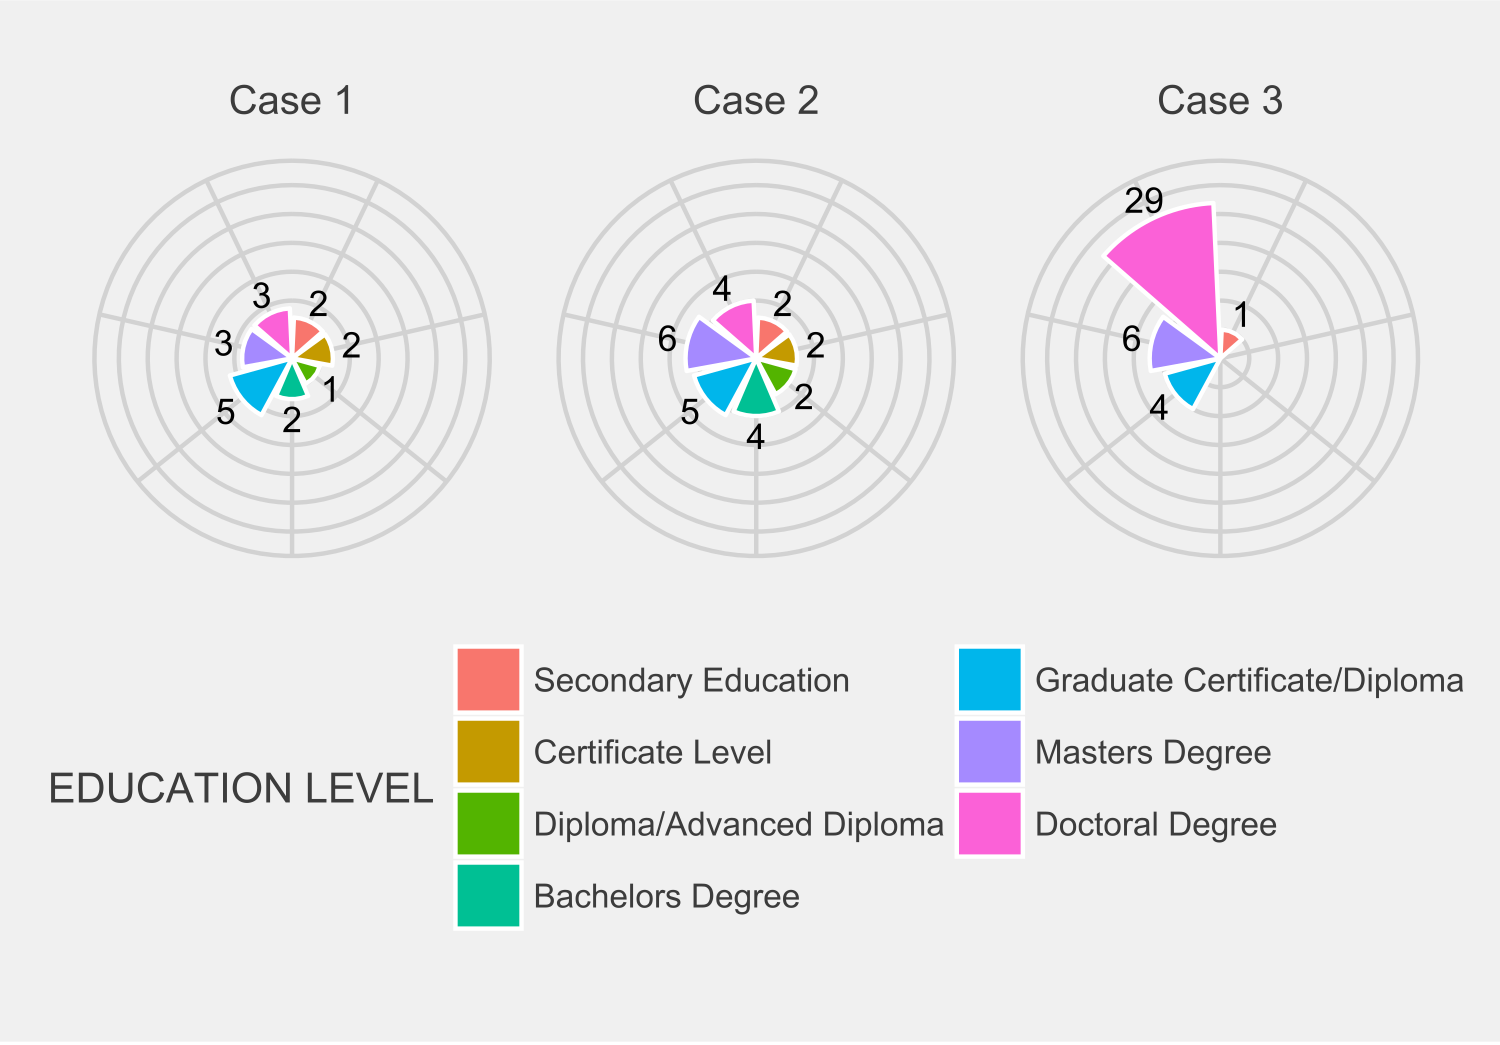
\includegraphics[width=0.7\linewidth]{Images/ed_level_rose}
	\caption{Breakdown of educational level in each case}
	\label{fig:edlevelrose}
\end{figure}

\begin{figure}
	\centering
	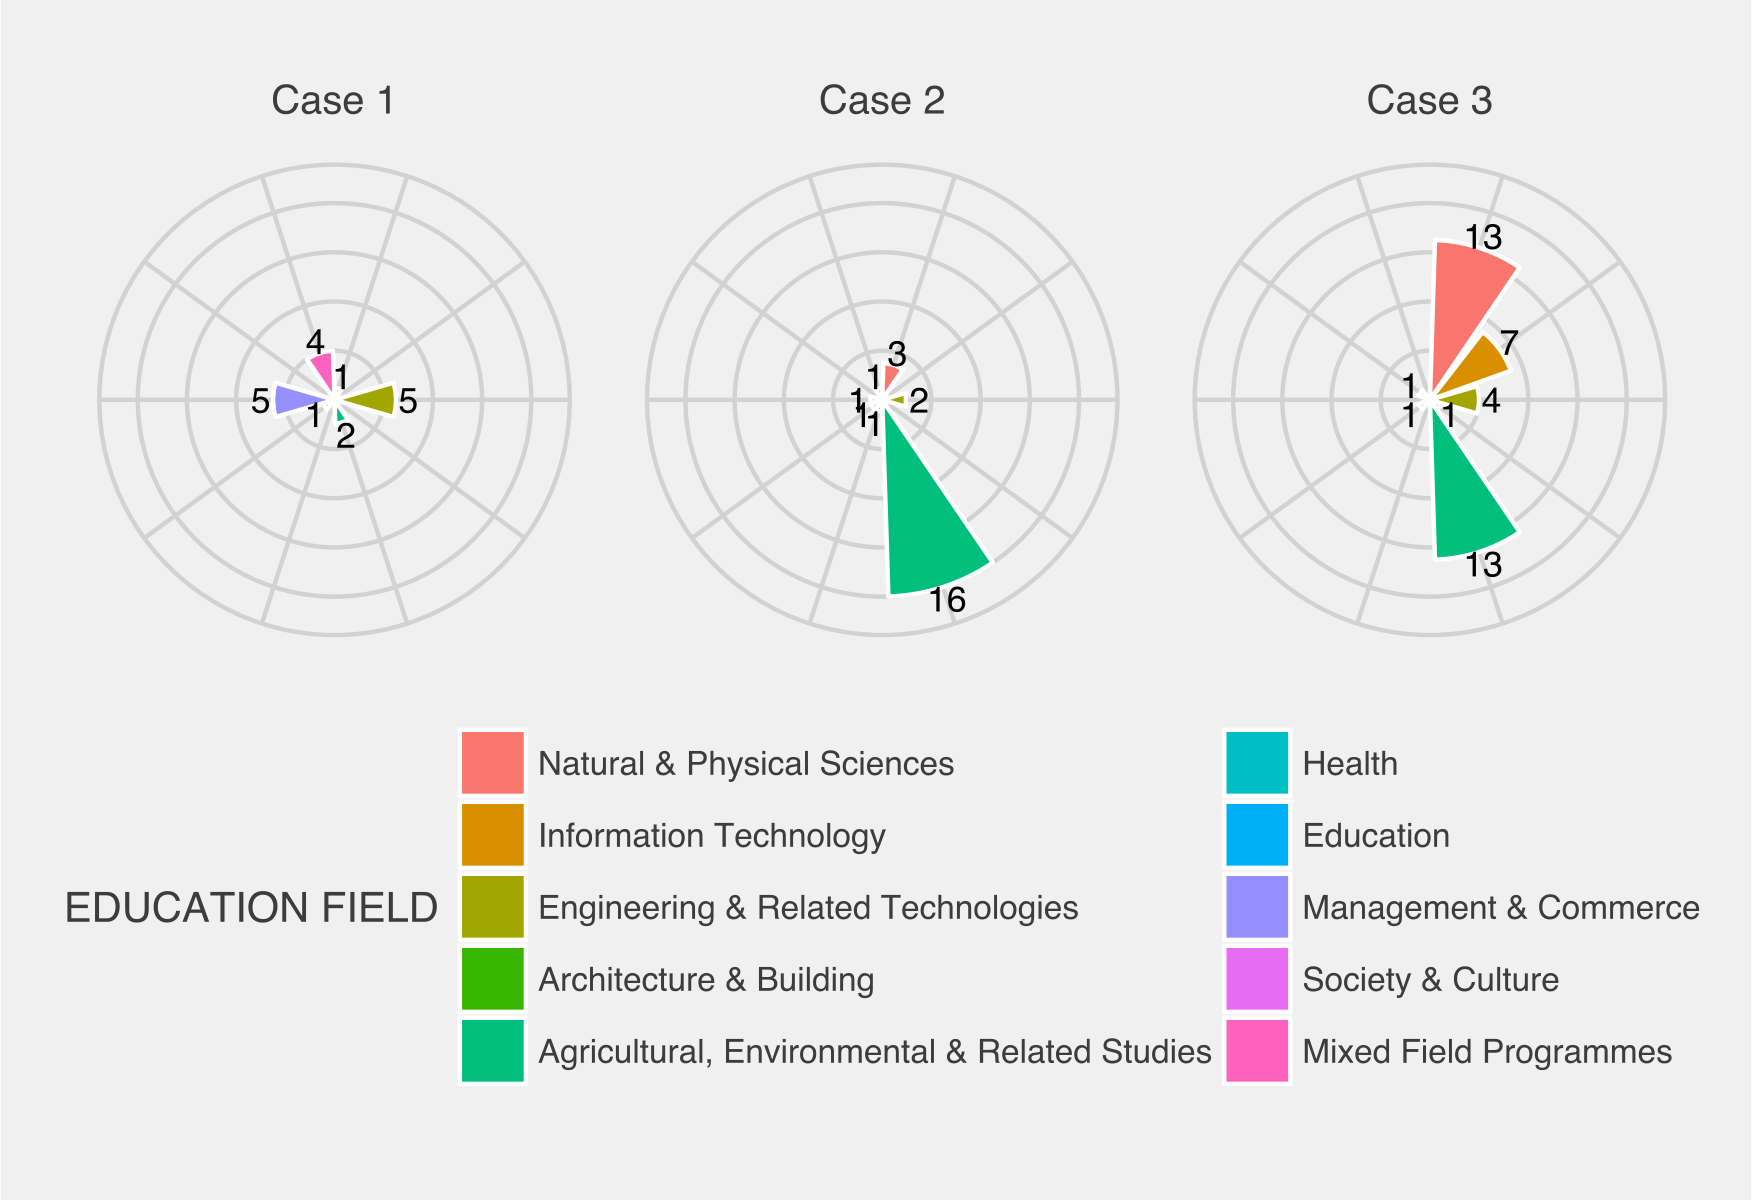
\includegraphics[width=0.7\linewidth]{Images/ed_field_rose}
	\caption{Breakdown of broad education field in each case}
	\label{fig:edfieldrose}
\end{figure}